Un'altra parte fondamentale del progetto è il database, in quanto il sito si appoggia su di esso per richiedere informazioni.\\ 
In fase di progettazione è stato pensato di creare un database con la funzione di contenere tutti i dati relativi ai prodotti in vendita, ovvero \emph{paste} e \emph{torte}, e al contenuto del contenitore \emph{news}.\\
Come si può vedere dalla \emph{Figura \ref{Fig:schemadb}}, le tabelle (che rappresentano sià entità che associazioni e i loro relativi attributi chiave/non chiave) sono quattro:
\begin{itemize}
		\item \textbf{Prodotto:} contiene tutte i dati relativi ai prodotti che verranno visualizzati nelle pagine \emph{Paste} e \emph{Torte}
		\item \textbf{Recensione:} contiene tutti i dati riguardo al feedback rilasciato da un utente per un prodotto specifico
		\item \textbf{Utente:} contiene i dati di tutti gli utenti che sono registrati al sito della pasticceria
		\item \textbf{News:} contiene tutti i dati addetti a riempire la sezione \emph{News} sotto il menu 
\end{itemize} 
Per vari motivi che sono stati discussi all'interno del gruppo, tre delle quattro tabelle elencate sono utilizzate nel momento in cui PHP interviene per prelevare i dati di interesse dal database.\\
Come spiegato nella sezione \emph{Analisi}, esistono due tipi di utenti in questo progetto: \emph{utente generico} e \emph{amministratore}.\\ L'utente generico non viene salvato nella tabella \emph{Utente}, in quanto non ha bisogno di registrarsi al sito per la semplice navigazione, mentre l'amministratore deve avere le credenziali appposite per entrare nell'\emph{Area amministratore}.\\
Inoltre, è obbligatorio l'utilizzo della tabella \emph{News} per visualizzare le novità della pasticceria, e della tabella \emph{Prodotto} per poter visualizzare paste e torte, in quanto i dati sono richiesti dinamicamente (altrimenti le pagine sarebbero vuote)\\
Ergo, la tabella \emph{Recensione} può servire solo nel caso in cui si vuole aggiungere un servizio interno al sito che prevede la registrazione di utenti che possono scrivere recensioni per i prodotti della pasticceria. Quindi, ai fini degli obiettivi del nostro progetto, la tabella, con l'intento di averla già pronta per implementazioni future.\\
Stesso discorso si applica alla tabella \emph{Utente}: in questo progetto, questa tabella sarà riempita solamente con i dati dell'amministratore, in quanto unico utente ad aver accesso all'\emph{Area amministratore} implementata nel sito.\\
\begin{figure}[!h]
	\centering
	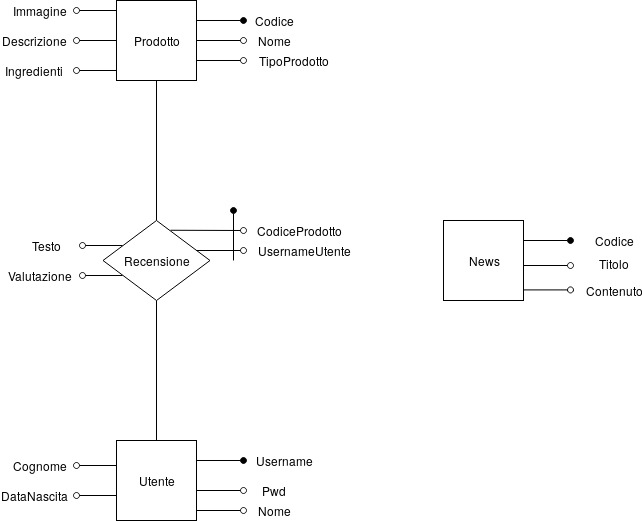
\includegraphics[width=0.7\linewidth]{sezioni/Progettazione/Immagini/schema_concettuale.jpg}
    \caption{Schema concettuale database}
	\label{Fig:schemadb}
\end{figure}